\section{Realisierung}

\subsection{Programmierumgebung / Programmierrichtlinien}
Als Programmierumgebung wird Visual Studio 2022 verwendet. Die App basiert auf dem .net Framework 6.0. Die Programmierrichtlinien sind die Standard-C\#-Richtlinien.
\begin{itemize}
  \item Klassen, Methodennamen und Properties in Pascal Case
  \item Argumente von Methoden in Camel Case
  \item fields von Properties beginnen mit einem Underscore
  \item Enum und Interface immer mit dem jeweiligen Prefix, E oder I
  \item Jede Klasse in einer Separaten Datei
\end{itemize}

\subsubsection{Verwendete NuGet-Pakete}
\begin{table}[H]
  \centering
  \settowidth\tymin{\textbf{MaterialDesignTheme}}
  \setlength\extrarowheight{2pt}
    \begin{tabulary}{1.0\textwidth}{|L|C|L|}
      \hline
      \rowcolor[HTML]{4473C5}\textbf{Paket} & \textbf{Version} & \textbf{Beschreibung}\\
    \hline
    \textbf{FontAwesome6. Svg} & 2.0.2 & SVG-Icon Bibliothek, wird für die Icons in der MenuBar verwendet.\\
    \hline
    \textbf{MaterialDesign MessageBox. SirTheta} & 1.1.3 & Eine Messagebox welche das Material Design Theme verwendet. Die Standard Messagebox passt nicht zu der sonst nach Material-Design aufgebauten Applikation. Dieses NuGet-Paket wurde von mir selber erstellt. Der Sourcecode dazu ist auf GitHub unter \href{https://github.com/sirtheta/MaterialDesignMessageBox}{https://github.com/sirtheta/MaterialDesignMessageBox} verfügbar und kann frei verwendet werden\\
    \hline
    \textbf{MaterialDesignTheme} & 4.5.0 & Wird für die GUI-Darstellung verwendet. Enthält Material Design Templates und Styles für WPF Controls in .NET\\
    \hline
    \textbf{Microsoft. EntityFrameWork Core} & 6.0.4 & Datenbank ORM. Wird für die Datenbankverwaltung verwendet\\
    \hline
    \textbf{Microsoft.EntityFrameWork Core.SqlServer} & 6.0.4 & Microsoft SQL Server database provider für Entity Framework Core\\
    \hline
    \textbf{Notifications. Wpf. Core} & 1.4.0 & Toast notifications für WPF apps. Wird zum Anzeigen von Toasts in der App verwendet \\
    \hline
    \textbf{Microsoft.Xaml. Behaviors.Wpf} & 1.1.39 & Behaviors für XAML. Wird z.B. für das Binding von einem Trigger, wie das Loaded Event verwendet\\
    \hline
\end{tabulary}
\caption{Verwendete NuGet-Pakete}
\end{table}

\newpage
\subsection{Softwareaufbau}
Die Applikation wird komplett im MVVM-Pattern aufgebaut. MVVM steht für Model-View-ViewModel. Mit diesem Konzept wird das View über DataBinding an das ViewModel gekoppelt, welches dann wiederum mit dem Model kommuniziert. 

\begin{figure}[H]
  \begin{center}
    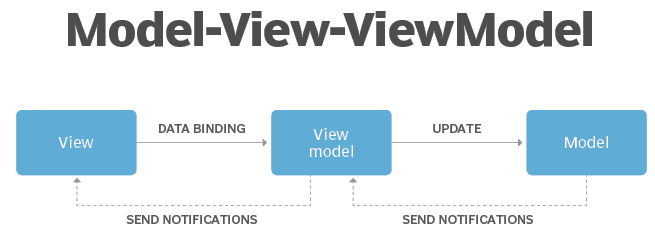
\includegraphics[width=0.6\linewidth]{content/images/mvvm.png}
    \caption{MVVM-Diagramm}
    \label{mvvm}
  \end{center}
\end{figure}

Somit besteht in der Applikation für jedes View ein ViewModel mit den entsprechenden Properties zum Anbinden an das View.\\
Um die Applikation Mehrsprachig zu gestalten, wurden alle Texte in einer Ressourcen-Datei erfasst. Für jede Sprache die unterstützt werden soll, muss eine solche Datei angelegt werden. Beim Start der Applikation wird je nach Systemsprache die entsprechende Sprachdatei geladen. Hierzu wurde ein override der ''OnStartup'' Methode gemacht, welches die Sprachdatei lädt. (Siehe App.xaml.cs) Im Aktuellen Stand der Applikation wird nur deutsch oder als Default Englisch genommen.\\
Für Demonstrationszwecke wurde ein Button im Side Menu implementiert, welcher es ermöglicht die Sprache zur Laufzeit zwischen Deutsch und Englisch umzuschalten. Für die Demonstration wurden jedoch nur die Sprachschlüssel der Menu Bar auf Englisch übersetzt.
 
\newpage
\subsection{GUI-Implementierung}
Das Main-GUI ist in drei Bereiche durch ein Grid aufgeteilt, wie in der Grafik \fref{guiGrid} zu sehen ist.

\begin{figure}[H]
  \begin{center}
    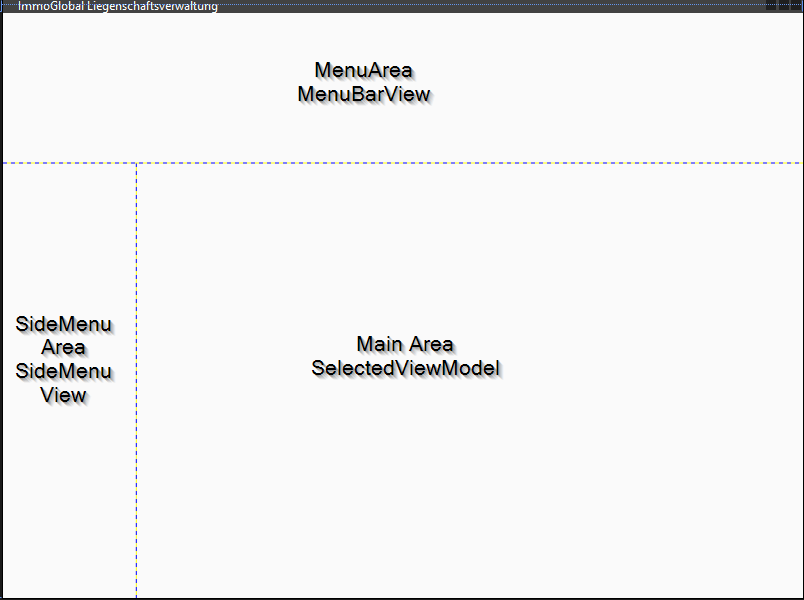
\includegraphics[width=0.6\linewidth]{content/images/MainGuiGrid.png}
    \caption{Main GUI Grid Aufbau}
    \label{guiGrid}
  \end{center}
\end{figure}
Die MenuArea und die SideMenuArea werden beim Start der Applikation durch das entsprechende ViewModel abgefüllt, und als Singleton-Instanz gehalten, auf welche immer über das MainWindowViewModel zugegriffen werden kann. Im seitlichen Menü werden je nach dem welches ViewModel in der MainArea geladen ist, die Buttons entsprechend angepasst und in der Menu Bar wird das Icon rot eingefärbt, wenn das entsprechende ViewModel in der MainArea geladen ist. So kann die Applikation sehr Dynamisch und übersichtlich gestaltet werden.
Alle Views bis auf das MainWindowView sind als UserControl definiert und können an beliebiger Stelle in der Applikation eingebunden werden, was das Wiederverwenden der Module deutlich vereinfacht.

\subsubsection{Namenskonzept für GUI-Komponenten}
Für das GUI werden verschieden Namen verwendet, welche hier beschrieben werden.
\begin{itemize}
  \item \textbf{DetailsView:} Definiert kleinere Module für Detailanzeigen wie z.B. die Detailanzeige für den Mieter
  \item \textbf{Menu:} Definiert die Menus
  \item \textbf{Overview:} Definiert die Views für die Übersichten
  \item \textbf{Upsert:} Definiert die Views für Update und Insert, z.B wird ein View zum Erstellen eines Mieters (Insert) und zum Anpassen eines Mieters verwendet.
\end{itemize}

\newpage
\subsection{Datenbankimplementierung und –anbindung}
\subsubsection{Generelles}
Die Datenbank wird mit dem Entity Framework Core mittels der Code-First Methode erstellt. In der \textbf{App.config} wird der Connection String für die Verbindung zur Datenbank festgelegt. Zum Testen und Vorführen der Applikation ist dieser auf die \verb+localdb+ eingestellt. Auch in der \textbf{App.config} Datei kann festgelegt werden, ob die Datenbank beim Start der Applikation gelöscht und mit Dummy-Einträgen gefüllt werden soll. So ist ein Vorführen und Testen der Applikation problemlos möglich.

\subsubsection{EF Core Datacontext}
Über die Klasse \verb+ImmoGlobalContext+  wird der Datacontext für Entity FrameWork Core erstellt. Jede Fachklasse wird mit dem \verb+DbSet+ implementiert und so werden die Tabellen dann von EF Core automatisch erzeugt und dann kann mittels des DbContext darauf zugegriffen werden. (EF Code First Methode)

\subsubsection{Audit Trail}
Um jede Änderung über die Applikation zu tracken, wurde ein Audit Trail implementiert. Jede Upsert-Methode verwendet anstelle des ImmoGlobalContext, den ImmoGlobalAuditableContext, welcher die \verb+SaveChanges()+ Methode des Entity Frameworks überschreibt und dann für jede veränderte Eigenschaft einen Eintrag in der AuditTrail Tabelle anlegt, mit dem aktuell eingeloggten User und dem Datum und der Zeit.
Aus Performancegründen wäre es bei einer Definitiven Applikation besser, wenn der Audit Trail direkt auf der Datenbank als Trigger erfasst werden würde.

\newpage
\subsection{Testprotokoll}
Automatisierte Tests wurden im Rahmen dieser Semesterarbeit keine umgesetzt. Für eine Real-World Applikation wären diese aber zwingend notwendig.

Hier werden als Testprotokoll alle in Kapitel \ref{testfaelle} definierten Testfälle mit ihrem Ist-Ergebnis dargestellt. Alle Testfälle wurden manuell durchgeführt

\begin{table}[H]
  \centering
  \settowidth\tymin{\textbf{Mietverträge}}
  \setlength\extrarowheight{2pt}
  \begin{tabulary}{1.0\textwidth}{|L|L|m{2cm}|}
    \hline
    \rowcolor[HTML]{fdebd0}
    \textbf{Testfall}& 
    \textbf{Soll} &
    \textbf{Ist}\\
    \hline
    In 10 Loginversuchen haben 3 ein Falsches Passwort und 3 kein Passwort & Alle 6 ungültigen Loginversuche werden erkannt, die 4 korrekten Loginversuche werden korrekt eingeloggt & \cellcolor[HTML]{02ce16} Erfolgreich\\
    \hline
    In 10 zu erfassenden Liegenschaften werden 3 Datensätze verwendet die nicht alle Muss-Daten enthalten & Die 7 korrekten Datensätze werden erfolgreich abgespeichert und die 3 ungültigen Datensätze werden mit einer Fehlermeldung abgewiesen & \cellcolor[HTML]{02ce16} Erfolgreich\\
    \hline
    In 10 zu erfassenden Objekten werden 3 Datensätze verwendet die nicht alle Muss-Daten enthalten & Die 7 korrekten Datensätze werden erfolgreich abgespeichert und die 3 ungültigen Datensätze werden mit einer Fehlermeldung abgewiesen & \cellcolor[HTML]{02ce16} Erfolgreich\\
    \hline
    In 10 zu erfassenden Mietverträgen werden 3 Datensätze verwendet die nicht alle Muss-Daten enthalten & Die 7 korrekten Datensätze werden erfolgreich abgespeichert und die 3 ungültigen Datensätze werden mit einer Fehlermeldung abgewiesen &\cellcolor[HTML]{02ce16} Erfolgreich\\
    \hline
    Es werden bei 10 Mietverträgen die Stati von nicht aktiv zu aktiv verändert und gespeichert & Bei allen 10 Mietverträgen wird der Status gültig gespeichert & \cellcolor[HTML]{02ce16} Erfolgreich\\
    \hline
    Es werden bei 10 Mietverträgen die Stati von aktiv zu nicht aktiv verändert und gespeichert & Bei allen 10 Mietverträgen wird der Status nicht aktiv gespeichert & \cellcolor[HTML]{02ce16} Erfolgreich\\
    \hline
    In einer Stichprobe werden 10 verschiedenen Objekte von unterschiedlichen Liegenschaften geladen & Es werden bei allen 10 Objekten die korrekten Daten der Mietverträge angezeigt. & \cellcolor[HTML]{02ce16} Erfolgreich\\
    \hline
    In einer Stichprobe werden 5 Mahnungen für Mieter und 5 Mahnungen für Kreditoren erstellt & Es können alle Mahnungen mit gültigen Daten erstellt werden &\cellcolor[HTML]{02ce16} Erfolgreich\\
    \hline
    Es werden 10 Rechnungen erstellt. Für 3 Rechnungen werden nicht alle Muss-Daten angegeben & Die 7 gültigen Rechnungen werden erfolgreich erstellt und dir 3 ungültigen werden mit einer Fehlermeldung abgewiesen & \cellcolor[HTML]{02ce16} Erfolgreich\\
    \hline   
    In einer Stichprobe werden 5 Rechnungen für Mieter und 5 Rechnungen für Kreditoren erstellt & Es können alle Rechnungen mit gültigen Daten erstellt werden & \cellcolor[HTML]{02ce16} Erfolgreich\\
    \hline
    Bei 10 zu erfassenden Kreditoren, werden 3 Datensätze verwendet, die nicht alle Muss-Daten enthalten & Die 7 korrekten Datensätze werden erfolgreich abgespeichert und die 3 ungültigen Datensätze werden mit einer Fehlermeldung abgewiesen & \cellcolor[HTML]{02ce16} Erfolgreich\\
    \hline
    Bei 10 zu erfassenden Mieter:innen, werden 3 Datensätze verwendet, die nicht alle Muss-Daten enthalten & Die 7 korrekten Datensätze werden erfolgreich abgespeichert und die 3 ungültigen Datensätze werden mit einer Fehlermeldung abgewiesen & \cellcolor[HTML]{02ce16} Erfolgreich\\
    \hline
  \end{tabulary}
  \caption{Testprotokoll}
\end{table}

\subsection{Deployment}
Als versuch für ein Deployment habe ich im DevOps eine BuildPipeline eingerichtet, welche ein Setup erstellt und dann als Artifact published, welches anschliessend heruntergeladen und Installiert werden kann. 

\subsubsection{Link zum Repository}
Die komplette Semesterarbeit ist unter diesem Link abrufbar: \href{https://dev.azure.com/michaelneuhaus/Semesterarbeit/}{Link zum DevOps Projekt}. Dort kann unter den Build Pipelines auch die kompilierte Dokumentation als PDF heruntergeladen werden.